%!TEX root = index.tex
\section{Développement}

% intro
% como era o time e do que cada pessoa era responsavel
% passo a passo da minha routine de dev
	% o que os outros faziam, o que eu fazia
% exemplo prático na criacao de alguma tela (das que geram relatorio).

Le deuxième mois de mon stage a été concentré sur le développement du système de gestion d'adhérents de CELGMED (Figure \ref{pp}). J'étais charge de la conception et création de plusieurs entités Java et fenêtres graphiques Flex, et par la liaison avec les bases de données SQL Server déjà existantes.

\begin{figure}[h]
\begin{center}
    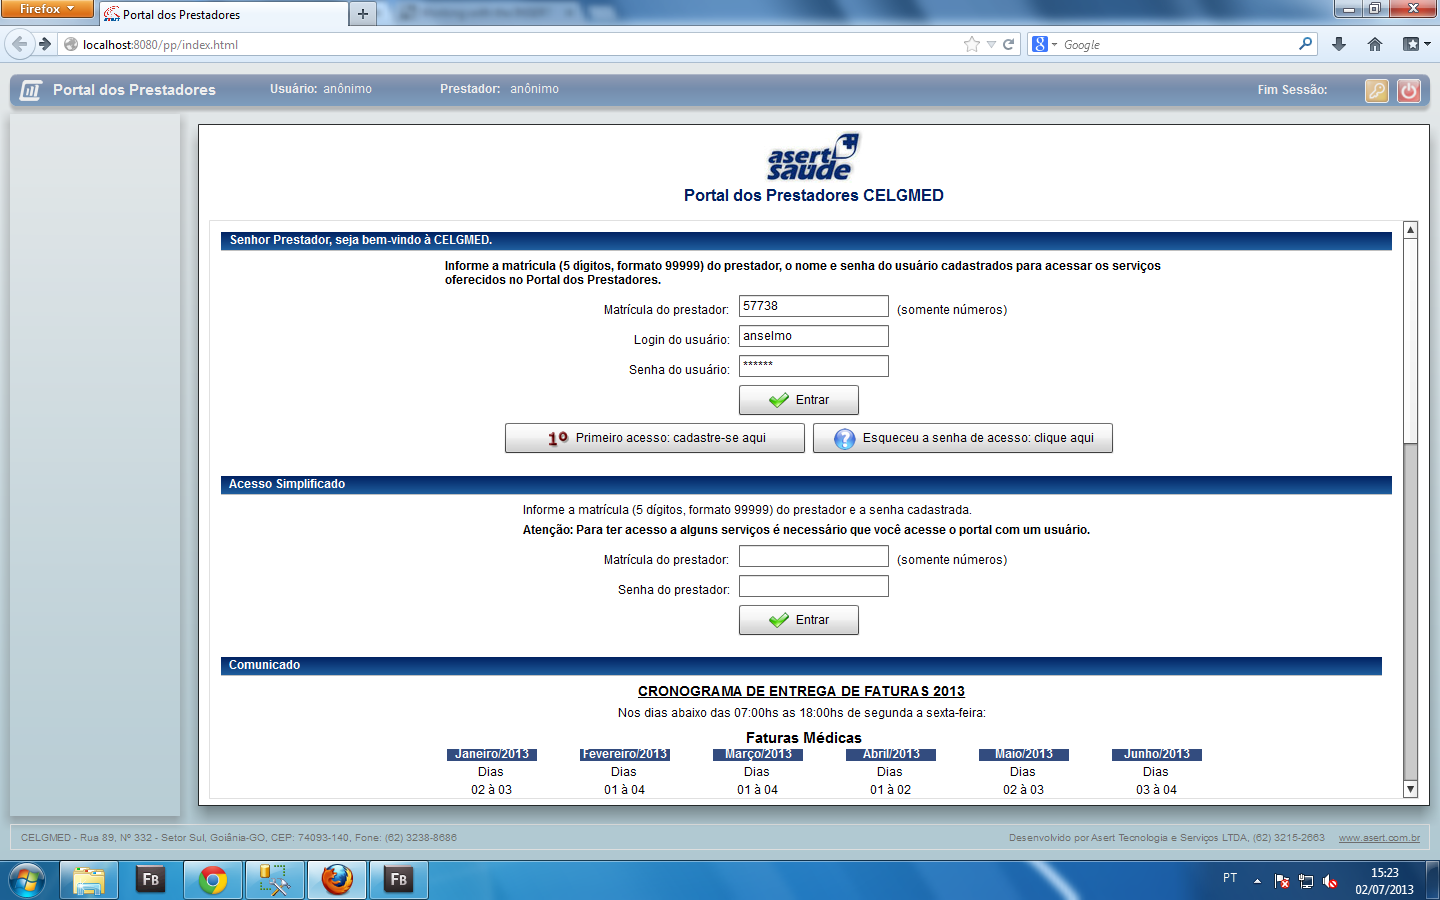
\includegraphics[scale=0.39]{img/pp}
    \caption{Page d'accueil du système d'adhérents CELGMED}
	\label{pp}
\end{center}
\end{figure}

L'équipe informatique était composé du chef de projets, d'un architecte logiciel, d'un développeur base de données, d'une analyste de systèmes, d'un développeur logiciel et de deux stagiaires, moi y compris. Du fait de n'être pas une équipe nombreuse, les tâches étaient souvent confondues et le développement était très agile : l'architecte logiciel touchait aussi au code, le développeur logiciel aidait le responsable des bases de données, et les stagiaires les aidait dans toutes les aires de la programmation.

De manière générale, afin de créer les fenêtres graphiques du système de gestion il fallait suivre quelques phases de développement, soit :

\begin{enumerate}
\item Création de la fenêtre graphique avec l'aide de l'éditeur visuel Adobe Flash Builder. Cette Vue était normalement associée à un ensemble d'entités plutôt qu'à une seule entité. Dans cette phase, il s'agissait d'une fenêtre de prototype, sans actions ou événements.
\item Vérification de quelles tables de la base de données (qui avaient déjà été créées dans la phase de conception) seraient utilisées dans l'application. Voir Section \ref{cycle}, Figure \ref{db}.
\item Création des entités correspondantes aux tables, c'est-à-dire, les classes de Contrôle, Business et Persistance correspondantes. Section \ref{framework}.
\item Codage des interrelations du flux de contrôle décrit dans la Table \ref{flux}. C'était ici que l'on peuplait la Vue avec les actions et événements, ainsi que les classes de \textit{C}, \textit{B} et \textit{P}. Section \ref{section-flux}.
\item Conception du rapport pdf à être généré sur iReport, dans le cas où la fenêtre le demandait, et intégration avec la Vue.
\item Vérification du code par le tuteur.
\end{enumerate}

\begin{figure}[h]
\begin{center}
    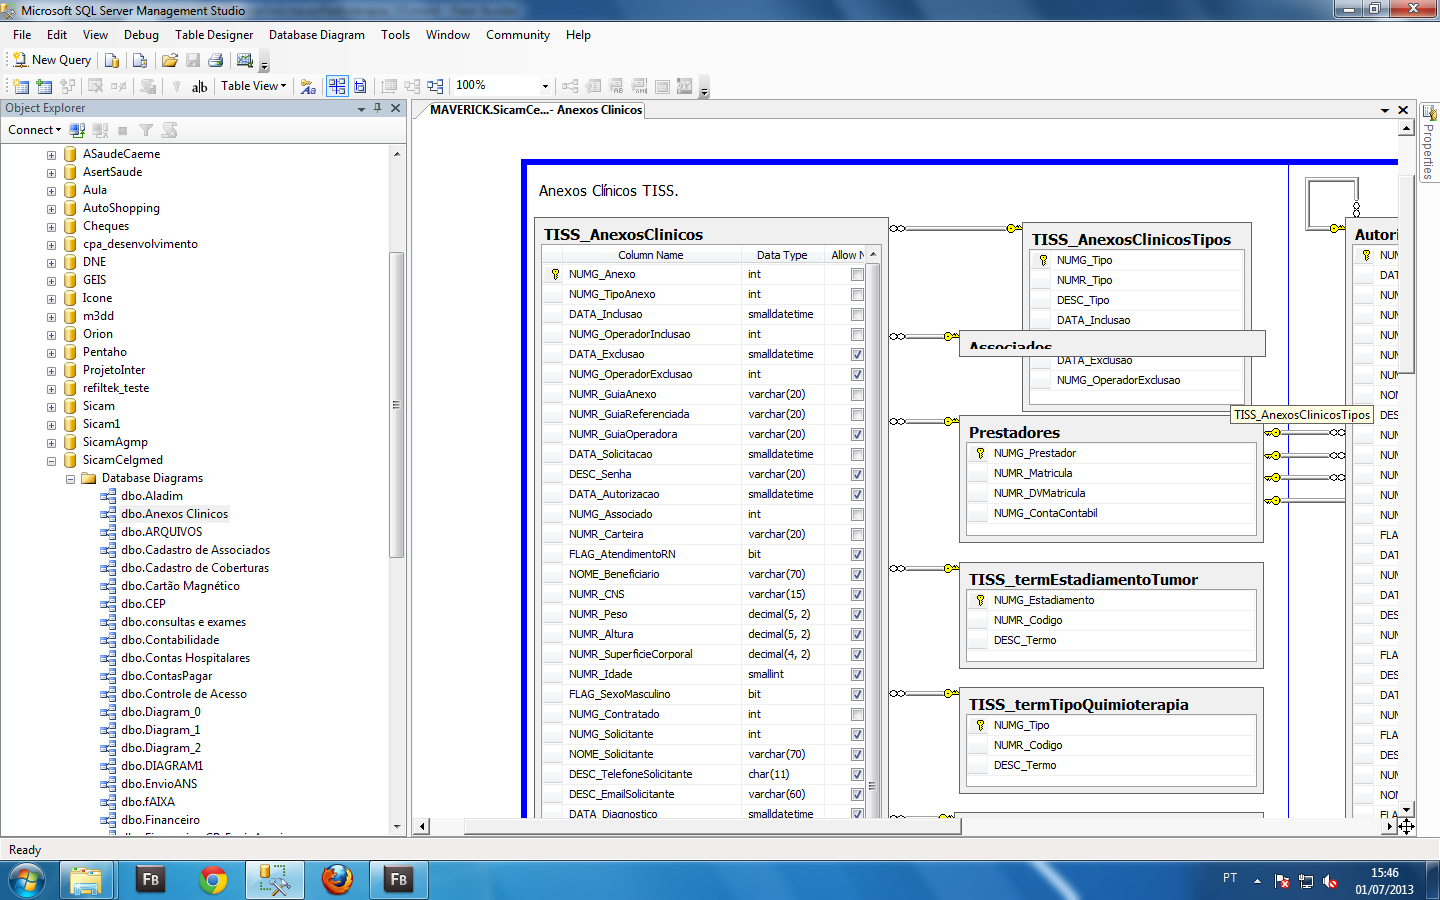
\includegraphics[scale=0.39]{img/db}
    \caption{Base de données relationnelles SQL Server}
	\label{db}
\end{center}
\end{figure}

Encore une fois, ces phases peuvent être mieux expliqués avec un example pratique que j'ai dû exécuter. Supposons la création d'une fenêtre graphique de demande de radiothérapie par un client de la mutuelle de santé CELGMED (Figure \ref{pp-radio}). Ces étapes deviennent donc :

\begin{enumerate}
\item Création de la fenêtre graphique avec l'aide de Flash Builder. Prise en compte des entités qui seraient utilisées : Bénéficiaire (la personne qui a demandé la radiothérapie), Médecin responsable, Maladies diagnostiquées, etc. L'élaboration de cette fenêtre de prototype était très vite, car on prenait souvent une autre fenêtre similaire comme modèle.
\item Vérification des tables à être utilisées : \texttt{celgmed.Beneficiaire}, \texttt{celgmed} \texttt{.Medecin}, \texttt{celgmed.Maladie}, etc.
\item Création des entités correspondantes aux tables : \underline{Ebeneficiaire}, \underline{Emedecin}, \underline{Emaladie}, ainsi que celles correspondantes à la radiothérapie proprement dite, \underline{Cradiotherapie}, \underline{Bradiotherapie}, \underline{Pradiotherapie}. 
\item Codage du flux de contrôle. Un clic dans le bouton « Sauvegarder » faisait que la vue appelle le Cradiotherapie, qui à son tour mettait en place le Bradiotherapie pour vérifier la logique associé à une sauvegarde de données, qui ensuite demandait que la Pradiotherapie fasse les altérations dans les tables avec des commandes SQL : ``\texttt{UPDATE \textit{celgmed.Beneficiaire} SET \textit{VISITE\_MEDICALE}=\textit{1} WHERE \textit{NOM\_BENEFICIAIRE}=`\textit{Pierre \\ Dubois}'}''. Le message d'erreur ou succès retournait à la fenêtre et l'utilisateur voyait le résultat de sa commande : ``Bénéficiaire mis à jour''. Celle-ci était l'étape la plus fastidieuse, car sa sous-division était beaucoup difficile ; la classe P nécessitait de la B, qui nécessitait de la C, qui à son tour était très lié à la V, et donc les fenêtres soit étaient finies, soit ne l'étaient pas.
\item Conception du rapport PDF à être généré. Il s'agissait de reproduire les mêmes éléments de la fenêtre graphique.
\item Vérification du code par le tuteur.
\end{enumerate}

\begin{figure}[h]
\begin{center}
    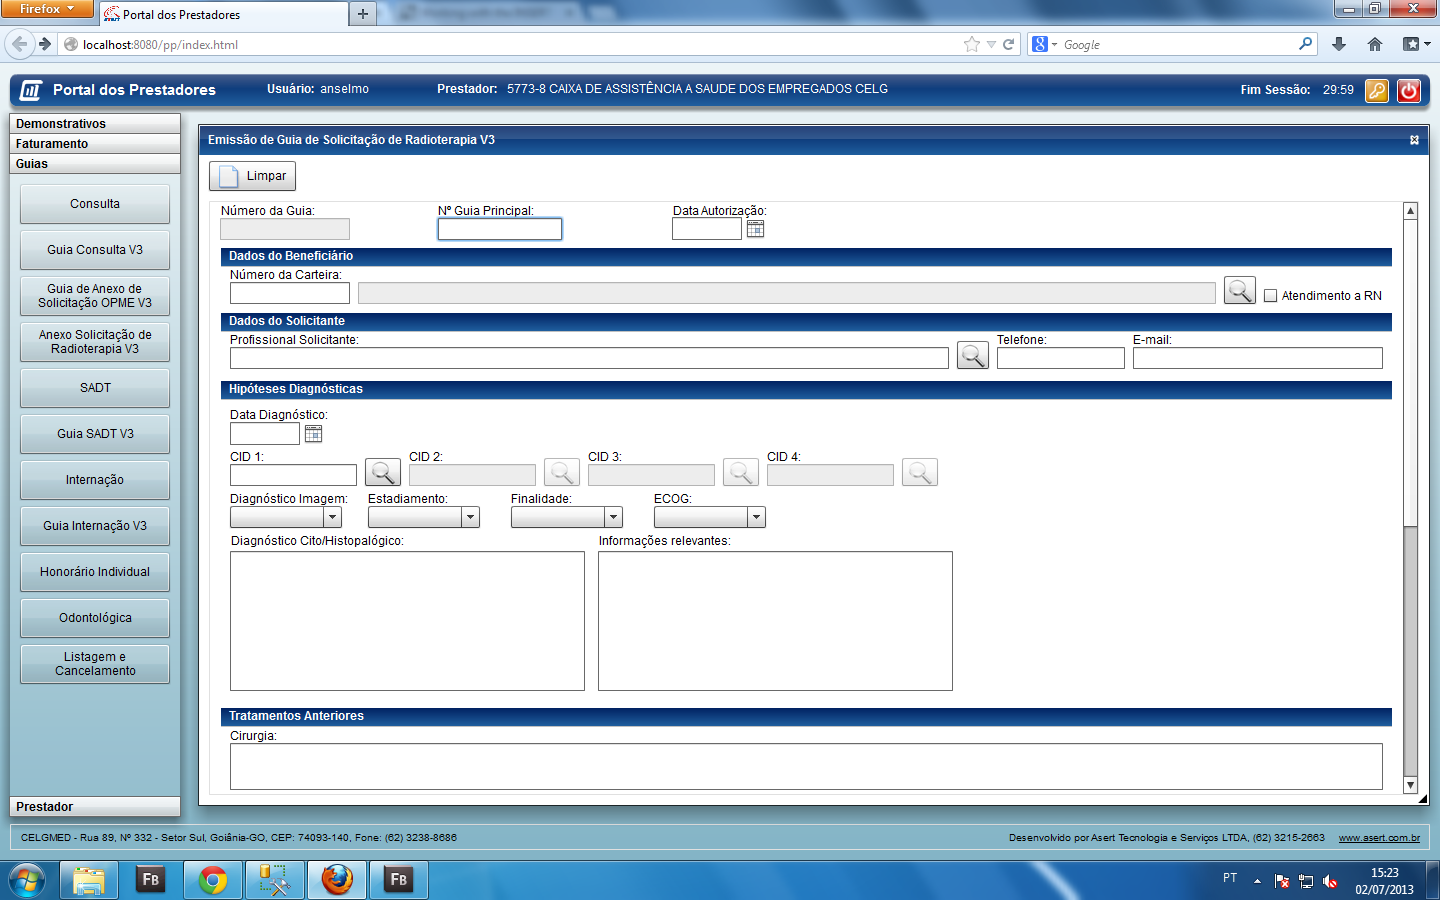
\includegraphics[scale=0.39]{img/pp-radio}
    \caption{Fenêtre de demande de radiothérapie}
	\label{pp-radio}
\end{center}
\end{figure}

Le développement de fenêtres plus élaborées, comme celle de la radiothérapie, prenait environ une semaine pour leur réalisation, alors que les fenêtres plus élémentaires, qui ne touchaient à une seule table de la base de données, comme dans l'enregistrement d'une Rue ou d'une Ville, comptaient une journée. Dans ce rythme, j'ai pu assister à la création de plus d'une dizaine de fenêtres complètes au cours du deuxième mois de mon stage.